%%%%%%%%%%%%%%%%%%%%%%%%%%%%%%%%%%%%%%%%%%%%%%%%%%%%%%%%%%%%%%%%%%%%%%%%%%%%%%%%
%2345678901234567890123456789012345678901234567890123456789012345678901234567890
%        1         2         3         4         5         6         7         8

\documentclass[letterpaper, 10 pt, conference]{ieeeconf}  % Comment this line out if you need a4paper

%\documentclass[a4paper, 10pt, conference]{ieeeconf}      % Use this line for a4 paper

\IEEEoverridecommandlockouts                              % This command is only needed if
                                                          % you want to use the \thanks command

\overrideIEEEmargins                                      % Needed to meet printer requirements.

%In case you encounter the following error:
%Error 1010 The PDF file may be corrupt (unable to open PDF file) OR
%Error 1000 An error occurred while parsing a contents stream. Unable to analyze the PDF file.
%This is a known problem with pdfLaTeX conversion filter. The file cannot be opened with acrobat reader
%Please use one of the alternatives below to circumvent this error by uncommenting one or the other
%\pdfobjcompresslevel=0
%\pdfminorversion=4

% See the \addtolength command later in the file to balance the column lengths
% on the last page of the document

% The following packages can be found on http:\\www.ctan.org
%\usepackage{graphics} % for pdf, bitmapped graphics files
%\usepackage{epsfig} % for postscript graphics files
%\usepackage{mathptmx} % assumes new font selection scheme installed
%\usepackage{times} % assumes new font selection scheme installed
%\usepackage{amsmath} % assumes amsmath package installed
%\usepackage{amssymb}  % assumes amsmath package installed

\usepackage{cite}
\usepackage{amsmath,amssymb,amsfonts}
\usepackage{algorithmic}
\usepackage{graphicx}
\usepackage{textcomp}
\usepackage{url}
\usepackage{multicol}
\usepackage{booktabs}
\newcommand{\tabitem}{~~\llap{\textbullet}~~}

\title{\LARGE \bf
C-ITS Architecture Framework
}


\author{Priyanka Karkhanis, Yanja Dajsuren and Mark van den Brand% <-this % stops a space
\thanks{Funded by European Union Commission , 723311.}%
\thanks{Priyanka is PhD candidate with Mathematics and Computer Science Department,
     Eindhoven University of Technology, Eindhoven, The Netherlands
        {\tt\small p.d.karkhanis@tue.nl}}%
\thanks{Yanja Dajsuren is an assistant professor and PDEng Program Director,
	 Eindhoven University of Technology, Eindhoven, The Netherlands
        {\tt\small Y.Dajsuren@tue.nl}}%
\thanks{Mark van den Brand is a professor at Mathematics and Computer Science Department,
  	 Eindhoven University of Technology, Eindhoven, The Netherlands
  	{\tt\small M.G.J.v.d.Brand@tue.nl}}%
}


\begin{document}



\maketitle
\thispagestyle{empty}
\pagestyle{empty}


%%%%%%%%%%%%%%%%%%%%%%%%%%%%%%%%%%%%%%%%%%%%%%%%%%%%%%%%%%%%%%%%%%%%%%%%%%%%%%%%
\begin{abstract}

Cooperative Intelligent Transport System (C-ITS) are Intelligent Transport Systems (ITS) where so-called ITS stations, such as vehicles, roadside equipment, traffic control centres and nomadic devices, communicate and share information. These complex and heterogeneous systems have their own independent usages. With continuous progress in the C-ITS domain, the convergence of these systems demands a strategy to coordinate and communicate efficiently. This initiative is currently demonstrated by the C-MobILE project. One of the objectives of C-MobILE is to define an integrated architecture based on a number of existing C-ITS architectures. Consolidating the existing C-ITS architectures into a generic standardized architecture requires a structured approach. A structured architecture framework is necessary for the integration of all the components of a C-ITS system.
In this paper, we describe an architecture framework, architecture viewpoints and a modelling approach for C-ITS systems. The objective of the architecture framework is to create a common language for system architects, stakeholders, and other roles in C-ITS. The architecture framework is intended to be used by eight existing C-MobILE deployment sites and to provide guidance for future projects.

\end{abstract}


%%%%%%%%%%%%%%%%%%%%%%%%%%%%%%%%%%%%%%%%%%%%%%%%%%%%%%%%%%%%%%%%%%%%%%%%%%%%%%%%
\section{INTRODUCTION}
The European industry has traditionally held a competitive position on a global scale in the field of Intelligent Transport Systems (ITS). While ITS focuses on intelligence at the roadside or in vehicles, Cooperative ITS (C-ITS) focuses on the communication between those systems. Such systems can be vehicles communicating with each other, with the infrastructure, or with other C-ITS systems. This interaction is where the term \emph{cooperative} comes from. There has been a tremendous amount of progress in the field of C-ITS. The C-ITS domain covers various fields such as software and systems engineering, traffic engineering, civil engineering, and information technology, which require a unified architecture. C-ITS is currently demonstrated by one of ongoing ITS projects name C-MobILE (Accelerating C-ITS Mobility Innovation and depLoyment in Europe)\footnote{C-MobILE: \url{http://c-mobile-project.eu/}}. C-MobILE is a large scale demonstration project spanning from 2017-2020. The C-MobILE aims for a fully safe and efficient road transport without casualties and serious injuries on European roads. To help achieve the C-MobILE goal, a well structured architecture, capable of being deployed to whole Europe is needed.

Within system and software engineering, the term architecture framework dates back to the 1970s. One can find numerous definitions on the World Wide Web; this one is representative \cite{zachman1} :
"An enterprise architecture framework, or architecture framework for short, is a prefabricated structure that you can use to organize your enterprise architecture into complementary views. (http://www.architectureframework.com/faq/) "

An architecture framework is determined by:
\begin{itemize}
	\item a set of architecture-related concerns;
	\item a set of stakeholders holding those concerns;
	\item a set of architecture viewpoints which frame (i.e., cover) those concerns; and
	\item a set of model correspondence rules.
\end{itemize}
We adapted architecture framework concepts to define C-MobIE architecture. To put the C-MobILE architecture framework concepts in context, we used the conceptual model of the ISO/IEC/IEEE 42010 international standard for architecture descriptions of systems and software\cite{arch_framework}, uses architecture viewpoints of the architecture framework for automotive systems\cite{yd} and concept of architecture perspective for shaping the architecture views\cite{woods}.


\section{Problem Statement}

Several C-ITS projects such as DTCIM, FREILOT, eCoMove, Compass4D, CO-GISTICS, CONVERGE have demonstrated the potential benefits of large-scale deployment. Most of these architectures have been designed with different objectives in mind, developed and deployed independently from each other. These architectures have their own multidisciplinary approach towards their deployed strategy. Such as in DTCIM architecture, sequence diagrams are used to show the interactions between actors, systems, interfaces etc. Other projects use ad-hoc notations and diagrams to depict the communication between systems and their components. These differences creates an inconsistent and inefficient behavior towards a seamless C-ITS implementation across various deployment sites. While these projects have been instrumental in the development and early, limited-scale deployment of C-ITS, they lack a common overall system architecture. This is the challenge the C-MobILE project aims to solve. One of the C-MobILE objective is to consolidate these existing architectures. Hence, a structured architecture is required by defining a standardized architecture framework and a common modelling language. This will help in having a common understanding between all stakeholders involved in C-MobILE.

\section{Related Work}

\section{Defining C-ITS Architecture Framework}

\section{Perspective}

\section{Applying C-ITS Arch Framework}

Here we shared the result of ref arch in context of c-mobile

As a well-defined architecture framework is considered to be an important part of any architecture description\cite{arch_desc}, we define an architecture framework for the C-ITS domain. To put architecture framework and architecture description concepts in context, we extend the conceptual model of the ISO/IEC/IEEE 42010 architecture framework as illustrated in \ref{arch_frmework}. The conceptual model of architecture framework is highlighted in blue and the relationships of architecture description concepts are added to the original standard diagram.

\begin{figure}[ht!]
	\centering
	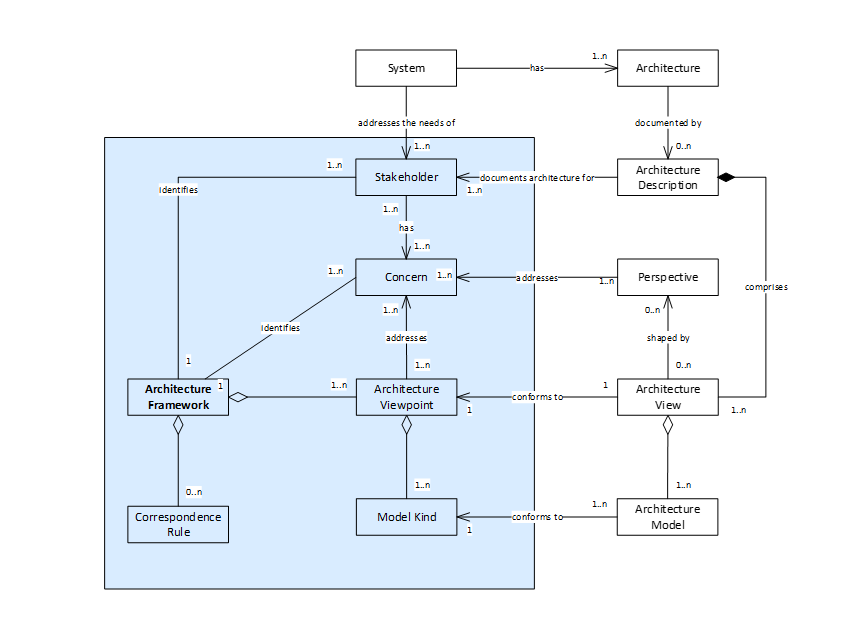
\includegraphics[width=0.47\textwidth]{arch_framework}
	\caption{Architecture Framework in Context}
	\label{arch_frmework}
	\centering
\end{figure}

As illustrated, an architecture description documents an architecture for the stakeholders using a set of Architecture Views and models. An Architecture View conforms to a viewpoint which addresses stakeholder concerns and can be shaped by a number of perspectives. The perspective defines concerns that guide architectural decision making to help ensure that the resulting architecture quality characteristics considered by the perspective \cite{woods}. This is essential for the C-ITS architectures as the architectural choices are costly to make after the implementation. In the existing C-ITS reference architectures, security is considered broadly albeit from limited aspects e.g. from the information and communication views. As described in the definition of an architecture framework, the C-ITS architecture framework specifies stakeholders, their concerns, viewpoints, model kinds, and correspondence rules.

\subsection{C-ITS Stakeholders and Concerns}

A stakeholder is an individual, team, or organization holding concerns for the system such as architect, designer, user, and authority \cite{iso42010}. A concern is any interest in the system such as functionality, structure, behaviour, and interoperability \cite{iso42010}. The C-ITS address the needs of some of following stakeholders. The rest of stakeholders description can be referred to C-MobILE Reference Architecture Report \cite{d31}.



\subsection{Viewpoints and Views}

We propose a set of six core viewpoints as part of the C-ITS architecture framework: Context, Functional, Information, Implementation, Physical, and Communication. These viewpoints are defined based on the existing literature and ITS reference architectures. We believe that this set of viewpoints enable structured architectural descriptions for the C-ITS. The relationships between views created using these viewpoints are shown in \ref{views_rel}. We believe that this set of viewpoints enable structured architectural descriptions for the C-ITS systems.

\begin{figure}[ht!]
	\centering
	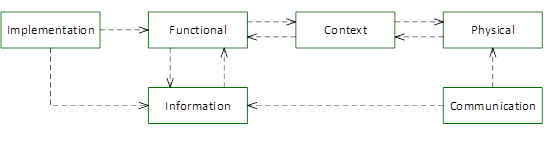
\includegraphics[width=0.47\textwidth]{views_rel}
	\caption{Relationships between architecture views}
	\label{views_rel}
	\centering
\end{figure}

Below table \ref{viewpoint_desc} briefly describes about viewpoint definitions and its respective views descriptions.

\begin{figure*}[t!]
	\centering
	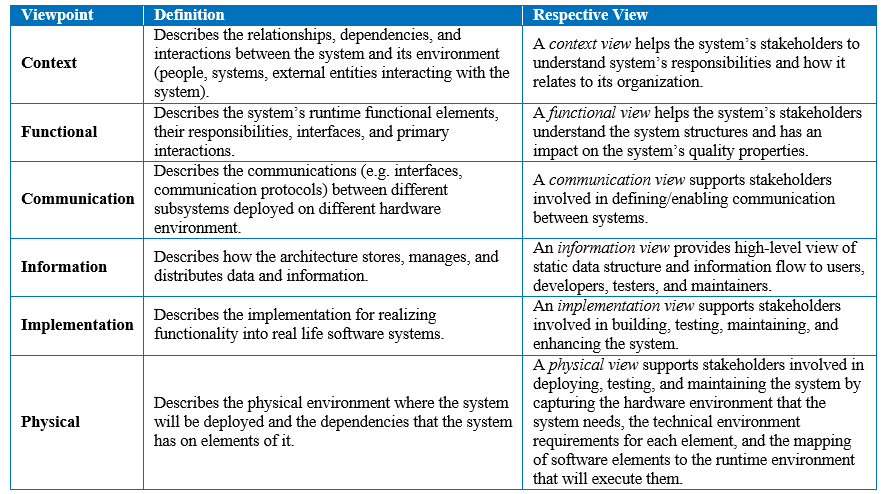
\includegraphics[width=0.80\textwidth]{viewpoint_desc}
	\caption{Viewpoints Description}
	\label{viewpoint_desc}
	\centering
\end{figure*}


\subsection{Architecture Perspective}
We identify the key perspectives for large scale demonstration of C-ITS systems. The identified perspectives can be applied to the views. Additional quality characteristics and perspectives may be added in the descriptions of concrete and implementation architectures. Architectural perspectives are used to formalize and guide the process of evaluating and reviewing the architectural models to ensure that the architecture satisfies the required quality characteristics and to select architectural tactics when it does not.
We summarize below the definitions of each perspective which are based on the international ISO/IEC 25010 standard\cite{quality}:

\begin{itemize}
	\item Interoperability is degree to which two or more systems, products or components can exchange information and use the information that has been exchanged.
	\item Security is degree to which a product or system protects information and data so that persons or other products or systems have the degree of data access appropriate to their types and levels of authorization.
	\item Performance efficiency is performance relative to the amount of resources used under stated conditions.
	\item Usability is degree to which a product or system can be used by specified users to achieve specified goals with effectiveness, efficiency and satisfaction in a specified context of use.
	\item Reliability is degree to which a system, product or component performs specified functions under specified conditions for a specified period.
	\item Availability is degree to which a system, product or component is operational and accessible when required for use.
	\item Adaptability is degree to which a product or system can effectively and efficiently be adapted for different or evolving hardware, software or other operational or usage environments.
\end{itemize}

We also provide architectural tactics for the interoperability and security perspectives so that they could be of use as an inspiration for elaborating the relevant tactics for the C-MobILE deployment architectures. Defining the perspectives for C-MobILE architecture definition and eventually large-scale demonstration of C-ITS systems would help avoid expensive changes in the later stages of development.

\subsection{Architecture Representation}
We propose to use Systems Modelling Language (SysML) diagram types to for architectural notations of the C-ITS architectures. The SysML is a general purpose modelling language for engineering systems and consists of structure diagram, requirement diagram, and behaviour diagram types as shown in \ref{sysml}.

\begin{figure}[ht!]
	\centering
	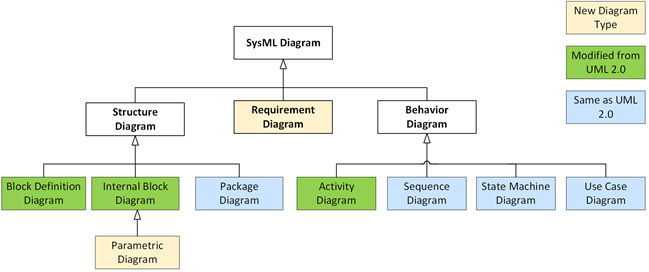
\includegraphics[width=0.47\textwidth]{sysml}
	\caption{SysML Types}
	\label{sysml}
	\centering
\end{figure}

\section{Result}

By adapting architecture framework and applying architecture descriptions, we defined reference architecure. The reference architecture provides a common vocabulary with which to discuss implementation, often with the aim to stress commonality often based on the generalizations of a set of solutions. The approach and methodology to extract reference architecture is described detail in "Defining C-ITS Reference Architecture" \cite{d31} <<WASA paper namee>>.

To develop a common and compatible reference architecture, we analyzed existing C-ITS reference architectures and projects that included the Dutch C-ITS Reference Architecture (DITCM) \cite{dtcim} <mention other architectures>. Besides these C-ITS architectures, we considered ITS implementations of the deployment sites involved with C-MobILE.

As an illustration of the architecture framework and reference architecture, we discuss here in detail the context viewpoint, view, and the context model.


\subsection{Context Viewpoint}

The context viewpoint describes the relationships, dependencies, and interactions between the system and its environment (e.g. people, systems and external entities) \cite{woods}. The context view conforms to the context viewpoint and helps system?s stakeholders (e.g. system/software architects, designers, developer and users) understand the system context.

\subsection{Context View}

The context view conforms to the context viewpoint. SysML Block Definition Diagram (BDD) is identified as suitable modelling notation for capturing the context viewpoint. SysML Use Case diagram can be used to show the usage of a system. The view conforms to viewpoint which satisfies the concerns of stakeholders as described in figure \ref{contextVP_view}.

\begin{figure*}[t!]
	\centering
	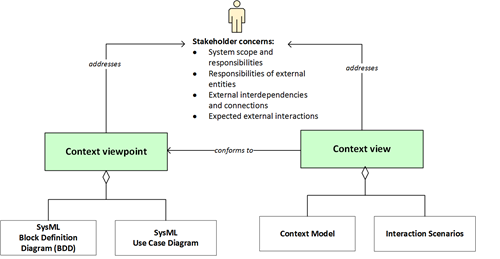
\includegraphics[width=0.80\textwidth]{contextVP_view}
	\caption{Context Viewpoint and Views}
	\label{contextVP_view}
	\centering
\end{figure*}

\subsection{Model Kinds}

The context diagram is the key model within a context view, placing the system in its environment by relating it to the external actors that it interacts with via explicit relationships that represent the connections to and from it. A context diagram is usually quite simple and contains elements of the following types:
\begin{itemize}
	\item System: the system being designed, which is treated as a black box, with its internal structure hidden.
	\item External Entities: systems, people, groups and other entities that the system interacts with.
	\item Connections: the interfaces, protocols, and connectors that link the external entities and the system being designed or utilized.
\end{itemize}

\subsubsection{Context Model}

The notations that we commonly see used for context diagrams are SysML Block Definition Diagram. C-MobILE consists of five main systems which is depicted as black box and corresponding actors?s connections with those systems is shown in Figure \ref{context_model}. The five main systems of the C-MobILE architecture are aligned with the five layers of the DITCM reference architecture \cite{dtcim}:

\begin{itemize}
	\item Support System: Comprise of sub-systems performing various tasks e.g.: governance, test and certification management, security and credentials management.
	\item Central System: Comprise of sub-systems to support connected vehicles, field and mobile devices. The sub-systems can be aggregated together or geographical or functionally distributed.
	\item Roadside System: Comprise of sub-systems which covers the ITS infrastructure on or along physical road infrastructure, e.g.: roadside units, signal/lane control etc.
	\item Vehicle System: Comprise of sub-systems which are integrated within vehicle such on-board systems (advanced driver assistance / safety systems, navigation, remote data collection or information).
	\item Traveler/VRU System: Comprise of both personal devices (e.g.: mobile devices, navigations devices) and specific systems connected to vehicles of VRU?s (e.g.: tags).
\end{itemize}

(Human) actors are treated as external entities that interact with the systems:

\begin{itemize}
	\item Vehicle Driver: An actor driving in a vehicle. The vehicle is a motorized vehicle (car, bus, truck) and not a vehicle of a vulnerable road user (bike, moped, motor). An actor in this category is directly concerned with Vehicle System as shown in Figure 24 through various vehicle related interfaces like : OBU , HMI etc.
	\item Vulnerable Road User: A VRU is a human actor like a pedestrian, cyclist or PTW driver; A motorcyclist is also an example of a PTW and is treated as a vulnerable road user in specific road hazard situations with other cars. An actor in this category is directly concerned with Traveler/VRU System as shown in Figure 24 through various interfaces like HMI, tablet, mobile, etc.
	\item  Road Operator: An actor responsible for the traffic management of a road network. An actor under this category is directly concerned with Roadside System through various communication channels and is responsible for collecting and evaluating data related to roadside information.
	\item Service Provider: An actor (organization) supplying services to one or more customers. Customers are either other organizations, including government (B2B / B2G / G2B / G2G) or end users (B2C / G2C). An actor under this category is directly concerned with Central System which also is responsible providing various services. Typical examples of a Service Provider are a Navigation Provider as a Service Provider providing navigation services to end users or organizations or a Traffic Information Provider as a Service Provider that provides road traffic related information, like traffic jams, incidents, road works warning etc.
\end{itemize}

\begin{figure*}[t!]
	\centering
	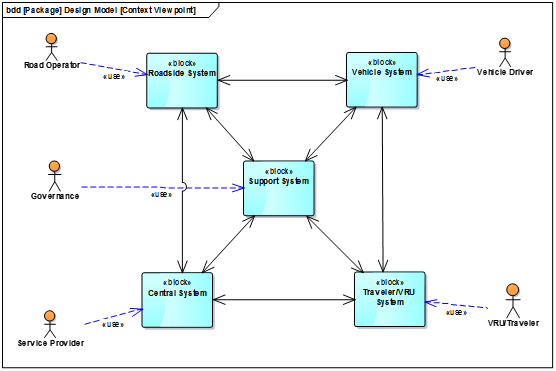
\includegraphics[width=0.80\textwidth]{context_model}
	\caption{Context model describing the relationship between systems and actors}
	\label{context_model}
	\centering
\end{figure*}

\subsection{Correspondence Rules}

The context viewpoint has correspondences with functional and physical viewpoints as highlighted in Figure \ref{correspondence_rules}. Functional and physical viewpoints have conformance correspondence to the context viewpoint.

\begin{figure}[ht!]
	\centering
	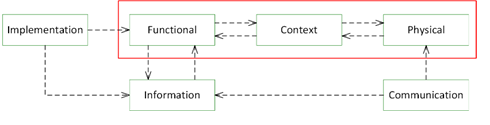
\includegraphics[width=0.47\textwidth]{correspondence_rules}
	\caption{Correspondence rules}
	\label{correspondence_rules}
	\centering
\end{figure}

Makse section for "Discussion"

Add

\section{CONCLUSIONS}

The main objective is to provide an architecture for the C-MobILE C-ITS environment. The purpose of this deliverable is to create a C-ITS reference architecture that enables pan-European interoperability of C-ITS architectures based on the generalization of existing C-ITS architectures. The C-ITS architecture framework and reference architecture is a first step in an integrated architecture based on a number of projects. We have analysed existing C-ITS architectures, especially CONVERGE, MOBiNET, and Dutch C-ITS Reference Architecture, to define common concepts and vocabulary for the C-MobILE architectures. The different architectures from the pilot sites are used as an input for defining a single homogeneous reference architecture in line with current standards.
The C-ITS architecture framework was developed by defining Architecture Viewpoints and their respective views addressing respective stakeholder concerns. This will facilitate the communication between different stakeholders. SysML is selected as a formal modelling language for describing the architectures. The architecture models are developed in Enterprise Architect using SysML profile. SysML block definition diagram is mainly used to create architectural models for different views.


\addtolength{\textheight}{-12cm}   % This command serves to balance the column lengths
                                  % on the last page of the document manually. It shortens
                                  % the textheight of the last page by a suitable amount.
                                  % This command does not take effect until the next page
                                  % so it should come on the page before the last. Make
                                  % sure that you do not shorten the textheight too much.

%%%%%%%%%%%%%%%%%%%%%%%%%%%%%%%%%%%%%%%%%%%%%%%%%%%%%%%%%%%%%%%%%%%%%%%%%%%%%%%%



\section*{ACKNOWLEDGMENT}

The C-MobILE project is funded by the European Union's Horizon 2020 research and innovation programme under grant agreement No 723311.


%%%%%%%%%%%%%%%%%%%%%%%%%%%%%%%%%%%%%%%%%%%%%%%%%%%%%%%%%%%%%%%%%%%%%%%%%%%%%%%%




\begin{thebibliography}{99}


\bibitem{iso42010} ISO/IEC/IEEE Systems and software engineering -- Architecture description," in ISO/IEC/IEEE 42010:2011(E) (Revision of ISO/IEC 42010:2007 and IEEE Std 1471-2000) , vol., no., pp.1-46, Dec. 1 2011 doi: 10.1109/IEEESTD.2011.6129467

\bibitem{kruchten}Kruchten, P.B. "The 4+ 1 view model of architecture." IEEE software 12.6 (1995): 42-50
\bibitem{togaf}Haren, Van. TOGAF Version 9.1. Van Haren Publishing, 2011.
\bibitem{zachman}Zachman, J. "The zachman framework for enterprise architecture." Zachman International 79 (2002).
\bibitem{arch_framework} ISO/IEC/IEEE 42010:2011. Systems and software engineering ? Architecture description. http://www.iso-architecture.org/
\bibitem{arch_desc}Emery, D., and Rich H. Every architecture description needs a framework: Expressing architecture frameworks using ISO/IEC 42010. Software Architecture, 2009 \& European Conference on Software Architecture. WICSA/ECSA 2009. Joint Working IEEE/IFIP Conference on. IEEE, 2009.
\bibitem{woods}Rozanski, N. and Woods, E. Software systems architecture: working with stakeholders using viewpoints and perspectives. Addison-Wesley, 2011.
\bibitem{yd}Dajsuren, Y. "On the design of an architecture framework and quality evaluation for automotive software systems." PhD thesis. Eindhoven University of Technology, 2015.
\bibitem{d31} Dajsuren, Y., Karkhanis, P., Kadiogullary, D. and Fuenfrocken, M. C-MobILE D3.1 Reference Architecture. Available at \url{http://c-mobile.diviprojects.wpengine.com/wp-content/uploads/sites/19/2018/03/C-MobILE-D3.1-ReferenceArchitecture_v0.1.pdf}
\bibitem{quality}International Organization for Standardization. ISO-IEC 25010: 2011 Systems and Software Engineering-Systems and Software Quality Requirements and Evaluation (SQuaRE)-System and Software Quality Models. ISO, 2011.
\bibitem{dtcim} van Sambeek, M. Turetken, O., Ophelders, F., Eshuis, R., Bijlsma, T. Traganos, K., Grefen. P (2015) Towards an Architecture for Cooperative ITS Applications in the Netherlands, Version 1.0. DITCM. April 17, 2015. Available at: https://goo.gl/pHSD9D
\bibitem{zachman1}Emery, D. and Hilliard, R., 2009, September. Every architecture description needs a framework: Expressing architecture frameworks using ISO/IEC 42010. In Software Architecture, 2009 \& European Conference on Software Architecture. WICSA/ECSA 2009. Joint Working IEEE/IFIP Conference on (pp. 31-40). IEEE.
\end{thebibliography}




\end{document}
